\iffalse
\documentclass[journal,12pt,twocolumn]{IEEEtran}
\usepackage{setspace}
\usepackage{gensymb}
\usepackage{xcolor}
\usepackage{caption}
\singlespacing
\usepackage{siunitx}
\usepackage[cmex10]{amsmath}
\usepackage{mathtools}
\usepackage{hyperref}
\usepackage{amsthm}
\usepackage{mathrsfs}
\usepackage{txfonts}
\usepackage{stfloats}
\usepackage{cite}
\usepackage{cases}
\usepackage{subfig}
\usepackage{longtable}
\usepackage{multirow}
\usepackage{enumitem}
\usepackage{bm}
\usepackage{mathtools}
\usepackage{listings}
\usepackage{tikz}
\usetikzlibrary{shapes,arrows,positioning}
\usepackage{circuitikz}
\renewcommand{\vec}[1]{\boldsymbol{\mathbf{#1}}}
\DeclareMathOperator*{\Res}{Res}
\renewcommand\thesection{\arabic{section}}
\renewcommand\thesubsection{\thesection.\arabic{subsection}}
\renewcommand\thesubsubsection{\thesubsection.\arabic{subsubsection}}

\renewcommand\thesectiondis{\arabic{section}}
\renewcommand\thesubsectiondis{\thesectiondis.\arabic{subsection}}
\renewcommand\thesubsubsectiondis{\thesubsectiondis.\arabic{subsubsection}}
\hyphenation{op-tical net-works semi-conduc-tor}

\lstset{
language=Python,
frame=single, 
breaklines=true,
columns=fullflexible
}
\begin{document}
\theoremstyle{definition}
\newtheorem{theorem}{Theorem}[section]
\newtheorem{problem}{Problem}
\newtheorem{proposition}{Proposition}[section]
\newtheorem{lemma}{Lemma}[section]
\newtheorem{corollary}[theorem]{Corollary}
\newtheorem{example}{Example}[section]
\newtheorem{definition}{Definition}[section]
\newcommand{\BEQA}{\begin{eqnarray}}
\newcommand{\EEQA}{\end{eqnarray}}
\newcommand{\define}{\stackrel{\triangle}{=}}
\newcommand{\myvec}[1]{\ensuremath{\begin{pmatrix}#1\end{pmatrix}}}
\newcommand{\mydet}[1]{\ensuremath{\begin{vmatrix}#1\end{vmatrix}}}
\bibliographystyle{IEEEtran}
\providecommand{\nCr}[2]{\,^{#1}C_{#2}} % nCr
\providecommand{\nPr}[2]{\,^{#1}P_{#2}} % nPr
\providecommand{\mbf}{\mathbf}
\providecommand{\pr}[1]{\ensuremath{\Pr\left(#1\right)}}
\providecommand{\qfunc}[1]{\ensuremath{Q\left(#1\right)}}
\providecommand{\sbrak}[1]{\ensuremath{{}\left[#1\right]}}
\providecommand{\lsbrak}[1]{\ensuremath{{}\left[#1\right.}}
\providecommand{\rsbrak}[1]{\ensuremath{{}\left.#1\right]}}
\providecommand{\brak}[1]{\ensuremath{\left(#1\right)}}
\providecommand{\lbrak}[1]{\ensuremath{\left(#1\right.}}
\providecommand{\rbrak}[1]{\ensuremath{\left.#1\right)}}
\providecommand{\cbrak}[1]{\ensuremath{\left\{#1\right\}}}
\providecommand{\lcbrak}[1]{\ensuremath{\left\{#1\right.}}
\providecommand{\rcbrak}[1]{\ensuremath{\left.#1\right\}}}
\theoremstyle{remark}
\newtheorem{rem}{Remark}
\newcommand{\sgn}{\mathop{\mathrm{sgn}}}
\newcommand{\rect}{\mathop{\mathrm{rect}}}
\newcommand{\sinc}{\mathop{\mathrm{sinc}}}
\providecommand{\abs}[1]{\left\vert#1\right\vert}
\providecommand{\res}[1]{\Res\displaylimits_{#1}} 
\providecommand{\norm}[1]{\lVert#1\rVert}
\providecommand{\mtx}[1]{\mathbf{#1}}
\providecommand{\mean}[1]{E\left[ #1 \right]}
\providecommand{\fourier}{\overset{\mathcal{F}}{ \rightleftharpoons}}
\providecommand{\ztrans}{\overset{\mathcal{Z}}{ \rightleftharpoons}}
\providecommand{\system}[1]{\overset{\mathcal{#1}}{ \longleftrightarrow}}
\newcommand{\solution}{\noindent \textbf{Solution: }}
\providecommand{\dec}[2]{\ensuremath{\overset{#1}{\underset{#2}{\gtrless}}}}
\let\StandardTheFigure\thefigure
\def\putbox#1#2#3{\makebox[0in][l]{\makebox[#1][l]{}\raisebox{\baselineskip}[0in][0in]{\raisebox{#2}[0in][0in]{#3}}}}
     \def\rightbox#1{\makebox[0in][r]{#1}}
     \def\centbox#1{\makebox[0in]{#1}}
     \def\topbox#1{\raisebox{-\baselineskip}[0in][0in]{#1}}
     \def\midbox#1{\raisebox{-0.5\baselineskip}[0in][0in]{#1}}

\vspace{3cm}
\title{Conic Assignment}
\author{Gautam Singh}
\maketitle
\bigskip

\begin{abstract}
    This document contains the solution to Question 20 of Exercise 3 in Chapter
    11 of the class 11 NCERT textbook.
\end{abstract}

\begin{enumerate}
    \item Find the equation of the ellipse whose major axis is the $x$-axis and
    center is the origin and passes through the points
    \begin{align}
        \vec{P} = \myvec{4\\3},\ \vec{Q} = \myvec{6\\2}
    \end{align}

    \solution 
\fi
		Let the equation of the conic with focus $\vec{F}$, directrix
    $\vec{n}^\top\vec{x} = c$ and eccentricity $e$ be
    \begin{align}
        \vec{x}^\top\vec{V}\vec{x} + 2\vec{u}^\top\vec{x} + f = 0
        \label{eq:chapters/11/11/3/20/conic-def}
    \end{align}
    where
    \begin{align}
        \vec{V} &\triangleq \norm{\vec{n}}^2\vec{I} - e^2\vec{n}\vec{n}^\top \label{eq:chapters/11/11/3/20/V-def} \\
        \vec{u} &\triangleq ce^2\vec{n} - \norm{\vec{n}}^2\vec{F} \label{eq:chapters/11/11/3/20/u-def} \\
        f &\triangleq \norm{\vec{n}}^2\norm{\vec{F}}^2 - c^2e^2 \label{eq:chapters/11/11/3/20/f-def}
    \end{align}
    Since the conic is an ellipse whose major axis is along the $x$-axis, we have
    \begin{align}
        \vec{n} = \myvec{1\\0}
    \end{align}
    Thus,
    \begin{align}
        \vec{V} = \myvec{1-e^2&0\\0&1} \label{eq:chapters/11/11/3/20/V-val} \\
        \vec{u} = ce^2\myvec{1\\0} - \vec{F} \label{eq:chapters/11/11/3/20/u-val} \\
        f = \norm{\vec{F}}^2 - c^2e^2 \label{eq:chapters/11/11/3/20/f-val}
    \end{align}
    The centre of the conic is given by
    \begin{align}
        \vec{c} = -\vec{V}^{-1}\vec{u}
        \label{eq:chapters/11/11/3/20/center}
    \end{align}
    Since $\vec{c} = \vec{0}$ and $\vec{V}^{-1} \neq \vec{0}$, it follows from 
    \eqref{eq:chapters/11/11/3/20/center} that $\vec{u} = \vec{0}$. Thus, from \eqref{eq:chapters/11/11/3/20/u-val},
    \begin{align}
        \vec{F} = \myvec{ce^2\\0}
        \label{eq:chapters/11/11/3/20/F-c-e}
    \end{align}
    and so,
    \begin{align}
        f = c^2e^2\brak{e^2-1}
        \label{eq:chapters/11/11/3/20/f-c-e}
    \end{align}
    Putting $\vec{x} = \vec{P}$ in \eqref{eq:chapters/11/11/3/20/conic-def} and using \eqref{eq:chapters/11/11/3/20/F-c-e}
    and \eqref{eq:chapters/11/11/3/20/f-c-e},
    \begin{align}
        \myvec{4&3}\myvec{1-e^2&0\\0&1}\myvec{4\\3} + f &= 0 \\
        \implies 16e^2 - f = 25 \label{eq:chapters/11/11/3/20/e1}
    \end{align}
    Putting $\vec{x} = \vec{Q}$ in \eqref{eq:chapters/11/11/3/20/conic-def}, we get
    \begin{align}
        \myvec{6&2}\myvec{1-e^2&0\\0&1}\myvec{6\\2} + f &= 0 \\
        \implies 36e^2 - f = 40 \label{eq:chapters/11/11/3/20/e2}
    \end{align}
    The equations \eqref{eq:chapters/11/11/3/20/e1} and \eqref{eq:chapters/11/11/3/20/e2} can be formulated as
    a matrix equation
    \begin{align}
        \myvec{16&-1\\36&-1}\myvec{e^2\\f} = \myvec{25\\40}
        \label{eq:chapters/11/11/3/20/mtx-eqn}
    \end{align}
    and can be solved using the augmented matrix.
    \begin{align}
        \myvec{16&-1&25\\36&-1&40} &\xleftrightarrow[]{R_1\leftarrow R_1-R_2} \myvec{-20&0&-15\\36&-1&40} \\
                 &\xleftrightarrow[]{\substack{R_1\leftarrow\frac{R_1}{-5}\\R_2\leftarrow -R_2}} \myvec{4&0&3\\-36&1&-40} \\
                 &\xleftrightarrow[]{R_2\leftarrow R_2+9R_1}\myvec{4&0&3\\0&1&-13} \\
                 &\xleftrightarrow[]{R_1\leftarrow\frac{R_1}{4}}\myvec{1&0&\frac{3}{4}\\0&1&-13}
    \end{align}
    Thus,
    \begin{align}
        e^2 = \frac{3}{4},\ f = -13
    \end{align}
    And the equation of the conic is given by
    \begin{align}
        \vec{x}^\top\myvec{\frac{1}{4}&0\\0&1}\vec{x} - 13 = 0
    \end{align}
    The situation is illustrated in Fig. \ref{fig:chapters/11/11/3/20/ellipse}
    \begin{figure}[!ht]
        \centering
        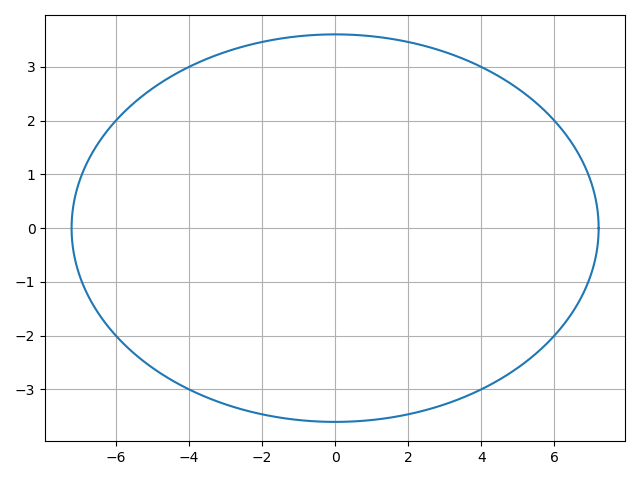
\includegraphics[width=\columnwidth]{chapters/11/11/3/20/figs/ellipse.png}
        \caption{Locus of the required ellipse.}
        \label{fig:chapters/11/11/3/20/ellipse}
    \end{figure}
